%%%%%%%%%%%%%%%%%%%%%%%%%%%%%%%%%%%%%%%%%%%%%%%%%%%%%%%%%%%%%%%%%%%%%%%%%%%%%%%%
\chapter{Обзор методов классификации и обнаружения транспортных средств с использованием методов технического зрения}
%%%%%%%%%%%%%%%%%%%%%%%%%%%%%%%%%%%%%%%%%%%%%%%%%%%%%%%%%%%%%%%%%%%%%%%%%%%%%%%%

%%%%%%%%%%%%%%%%%%%%%%%%%%%%%%%%%%%%%%%%%%%%%%%%%%%%%%%%%%%%%%%%%%%%%%%%%%%%%%%%
\section{Обнаружение транспортных средств по моделям (Model-Based Detection)}
%%%%%%%%%%%%%%%%%%%%%%%%%%%%%%%%%%%%%%%%%%%%%%%%%%%%%%%%%%%%%%%%%%%%%%%%%%%%%%%%

Обнаружение транспортных средств по модели осуществляется с использованием большой базы данных заранее подготовленных моделей. Во время работы этого метода, система пытается найти подходящую область в заданных кадрах пользуясь информацией из базы моделей. Для определения совпадения задается некоторый порог. Если результат сравнения между моделью и областью в кадре больше, чем заданный порог, тогда эта область будет определена как транспортное средство. Пример работы такого метода можно наблюдать на рисунке ниже.

\begin{figure}[htbp]
\centering
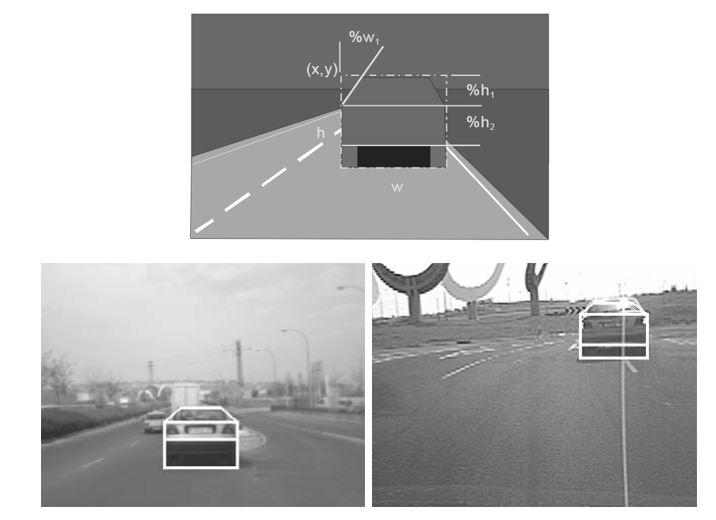
\includegraphics[width=0.5\textwidth]{image001.jpg}
\caption{Пример обнаружения по модели~\cite{one}}%
\label{fig:how-to-do-research}
\end{figure}

%%%%%%%%%%%%%%%%%%%%%%%%%%%%%%%%%%%%%%%%%%%%%%%%%%%%%%%%%%%%%%%%%%%%%%%%%%%%%%%%
\section{Обнаружение транспортных средств методами машинного обучения}
%%%%%%%%%%%%%%%%%%%%%%%%%%%%%%%%%%%%%%%%%%%%%%%%%%%%%%%%%%%%%%%%%%%%%%%%%%%%%%%%

Есть определенные особенности транспортных средств, которые позволяют отличить их от других объектов на изображении (грани, тени, симметрия). В ходе обнаружения, последовательно осуществляется поиск подобных характерных признаков на всем изображении. Минусы подобных алгоритмов заключаются в том, что если один из признаков отсутствует на изображении, то объект не может быть обнаружен. Также существует высокая вероятность ложного срабатывания.

В методах, основанных на классификаторах по признакам, транспортное средство рассматривается как единое целое. Процесс обнаружения заключается в выделении области, в которой находится транспортное средство. Для каждого кадра производится разделение изображения на несколько регионов. Процесс разделения определяется размером искомых признаков. После выполнения деления, выполняется извлечение признаков из каждого региона (гистограмма направленных градиентов ~(HOG), признаки Хаара, локальные бинарные оттенки ~(LBP)). Для выполнения классификации по признакам используются специальные классификаторы. Для использования этого метода необходимо правильно выбрать признаки, которые лучшим образом описывают транспортное средство. Из-за большого количества вариаций углов обзора это становится сложной задачей.
\nomenclature{HOG}{Histogram of Oriented Gradients}
\nomenclature{LBP}{Local binary patterns}

%%%%%%%%%%%%%%%%%%%%%%%%%%%%%%%%%%%%%%%%%%%%%%%%%%%%%%%%%%%%%%%%%%%%%%%%%%%%%%%%
\subsection{Способы извлечения признаков}
%%%%%%%%%%%%%%%%%%%%%%%%%%%%%%%%%%%%%%%%%%%%%%%%%%%%%%%%%%%%%%%%%%%%%%%%%%%%%%%%

%%%%%%%%%%%%%%%%%%%%%%%%%%%%%%%%%%%%%%%%%%%%%%%%%%%%%%%%%%%%%%%%%%%%%%%%%%%%%%%%
\subsubsection{Признаки Хаара}
%%%%%%%%%%%%%%%%%%%%%%%%%%%%%%%%%%%%%%%%%%%%%%%%%%%%%%%%%%%%%%%%%%%%%%%%%%%%%%%%

Признаки Хаара можно посчитать несколькими методами. Например, можно использовать горизонтальные и вертикальные прямоугольники или квадратный набор прямоугольников, что проиллюстрировано на рисунке ниже.

\begin{figure}[htbp]
\centering
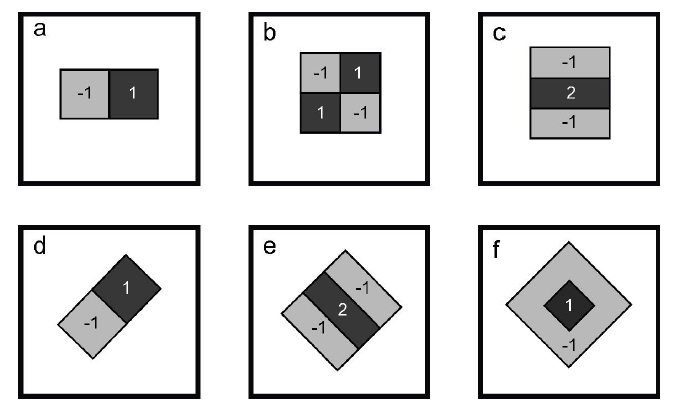
\includegraphics[width=0.5\textwidth]{image003.png}
\caption{Признаки Хаара~\cite{two}}%
\label{fig:how-to-do-research}
\end{figure}

Простейший прямоугольный признак Хаара можно определить~\cite{two}, как разность сумм пикселей двух смежных областей внутри прямоугольника, который может занимать различные положения и масштабы на изображении. Такой вид признаков называется 2-прямоугольным. Виола и Джонс~\cite{three} так же определили 3-прямоугольные и 4-прямоугольные признаки. Каждый признак может показать наличие (или отсутствие) какой-либо конкретной характеристики изображения, такой как границы или изменение текстур. Например, 2-прямоугольный признак может показать, где находится граница между темным и светлым регионами.

Линхарт и Майд~\cite{four} представили идею наклоненных (45$^{\circ}$ градусов) признаков Хаара. Это было сделано для увеличения размерности пространства признаков. Способ оказался удачным и некоторые наклонные признаки были способны лучше описывать объект. Например, 2-прямоугольный наклонный признак Хаара может показать наличие края, наклоненного на 45$^{\circ}$ градусов.

Мессом и Барзак~\cite{five} дополнили концепцию наклонных признаков Хаара. Хоть идея и является математически верной, на практике при использовании признаков под разными углами возникают проблемы. Для ускорения вычислений, алгоритм обнаружения использует изображения низкого разрешения, что приводит к ошибке округления. Исходя из этого, наклонные признаки Хаара обычно не используются.

%%%%%%%%%%%%%%%%%%%%%%%%%%%%%%%%%%%%%%%%%%%%%%%%%%%%%%%%%%%%%%%%%%%%%%%%%%%%%%%%
\subsubsection{Локальные бинарные оттенки (Local binary patterns)}
%%%%%%%%%%%%%%%%%%%%%%%%%%%%%%%%%%%%%%%%%%%%%%%%%%%%%%%%%%%%%%%%%%%%%%%%%%%%%%%%

Расчет признаков LBP происходит на сетке пикселей изображения. Значение каждого пикселя вокруг центрального сравнивается со значением центрального и заменяется либо единицей, либо нулем в зависимости от результата сравнения. После этого, как показано на рисунке ниже, все пиксели складываются с некоторыми коэффициентами и получается число. Разряды полученного числа описывают направления изменения яркости в изображении.

\begin{figure}[htbp]
\centering
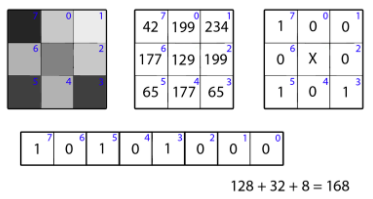
\includegraphics[width=0.5\textwidth]{image004.png}
\caption{Иллюстрация извлечения LBP признаков~\cite{six}}%
\label{fig:how-to-do-research}
\end{figure}

%%%%%%%%%%%%%%%%%%%%%%%%%%%%%%%%%%%%%%%%%%%%%%%%%%%%%%%%%%%%%%%%%%%%%%%%%%%%%%%%
\subsubsection{Гистограмма направленных градиентов (Histogram of Oriented Gradients)}
%%%%%%%%%%%%%%%%%%%%%%%%%%%%%%%%%%%%%%%%%%%%%%%%%%%%%%%%%%%%%%%%%%%%%%%%%%%%%%%%

Извлечение HOG признаков можно разделить на несколько шагов~\cite{seven}. Первым шагом вычислений во многих алгоритмах обнаружения особых точек является нормализация цвета и гамма-коррекция. На следующем шаге вычисляются гистограммы ячеек. Каждый пиксел в ячейке участвует во взвешенном голосовании для каналов гистограммы направлений, основанном на значении градиентов. Ячейки могут быть прямоугольной или круглой формы, каналы гистограммы равномерно распределяются от 0 до 180$^{\circ}$ или же от 0 до 360$^{\circ}$, в зависимости от того, вычисляется «знаковый» или «беззнаковый градиент». Далал и Триггс обнаружили, что беззнаковый градиент совместно с девятью каналами гистограммы дает лучшие результаты при распознавании людей. При распределении весов в голосовании вес пикселя может задаваться либо абсолютным значением градиента, либо некоторой функцией от него; в реальных тестах абсолютное значение градиента дает лучшие результаты. Другими возможными вариантами могут быть квадратный корень, квадрат или урезанное абсолютное значение градиента.

Для принятия во внимание яркости и контрастности градиенты следует локально нормировать, для чего ячейки нужно сгруппировать в более крупные связные блоки. Дескриптор HOG, таким образом, является вектором компонент нормированных гистограмм ячеек из всех областей блока. Как правило, блоки перекрываются, то есть каждая ячейка входит более чем в один конечный дескриптор. Используются две основные геометрии блока: прямоугольные ~(R-HOG) и круглые ~(C-HOG). Как можно видеть на рисунке ниже, блоки R-HOG обычно являются квадратными сетками, характеризующимися тремя параметрами: количеством ячеек на блок, количеством пикселов на ячейку и количеством каналов на гистограмму ячейки.
\nomenclature{R-HOG}{Rectangle Histogram of Oriented Gradients}
\nomenclature{C-HOG}{Circular Histogram of Oriented Gradients}

\begin{figure}[htbp]
\centering
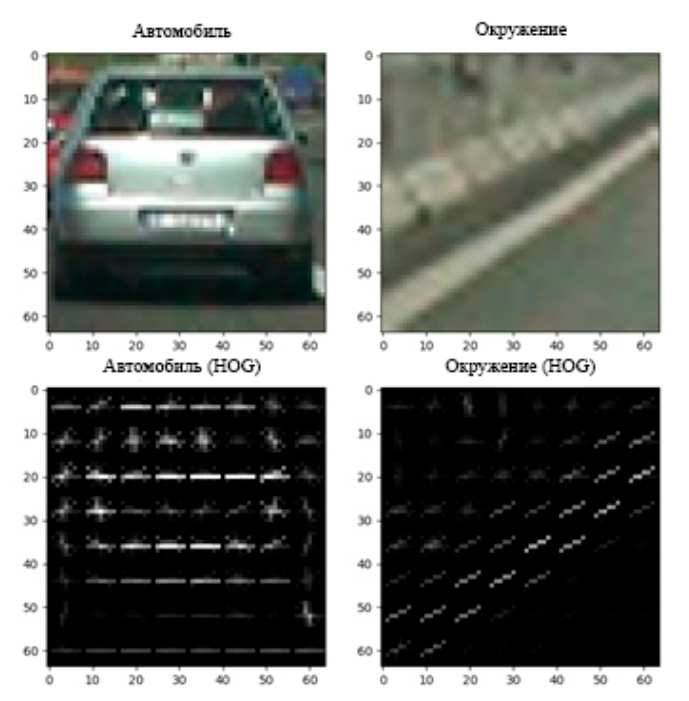
\includegraphics[width=0.5\textwidth]{image005.jpg}
\caption{Иллюстрация HOG-признаков~\cite{eight}}%
\label{fig:how-to-do-research}
\end{figure}

%%%%%%%%%%%%%%%%%%%%%%%%%%%%%%%%%%%%%%%%%%%%%%%%%%%%%%%%%%%%%%%%%%%%%%%%%%%%%%%%
\subsection{Классификация методом опорных веторов (Support Vector Machine)}
%%%%%%%%%%%%%%%%%%%%%%%%%%%%%%%%%%%%%%%%%%%%%%%%%%%%%%%%%%%%%%%%%%%%%%%%%%%%%%%%

Метод опорных векторов ~(SVM) — набор алгоритмов обучения с учителем, использующихся для задач классификации и регрессионного анализа. Принадлежит семейству линейных классификаторов. Особым свойством метода опорных векторов является непрерывное уменьшение эмпирической ошибки классификации и увеличение зазора, поэтому метод также известен как метод классификатора с максимальным зазором.
\nomenclature{SVM}{Support Vector Machine}

В алгоритмах машинного обучения возникает необходимость классифицировать данные. Каждый объект данных представляется как вектор (точка) в \(p\)-мерном пространстве (упорядоченный набор \(p\) чисел). Каждая из этих точек принадлежит только одному из двух классов. Вопрос состоит в том, можно ли разделить точки гиперплоскостью размерности \(p-1\). Это — типичный случай линейной разделимости. Искомых гиперплоскостей может быть много, поэтому полагают, что максимизация зазора между классами способствует более уверенной классификации. То есть, можно ли найти такую гиперплоскость, чтобы расстояние от неё до ближайшей точки было максимальным. Это эквивалентно тому, что сумма расстояний до гиперплоскости от двух ближайших к ней точек, лежащих по разные стороны от неё, максимальна. Если такая гиперплоскость существует, она называется оптимальной разделяющей гиперплоскостью, а соответствующий ей линейный классификатор называется оптимально разделяющим классификатором.

\begin{figure}[htbp]
\centering
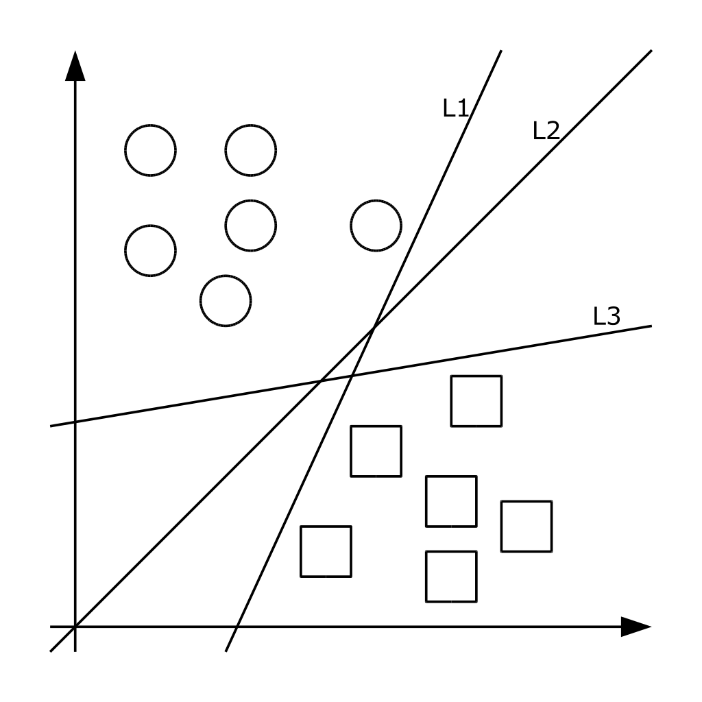
\includegraphics[width=0.5\textwidth]{image006.png}
\caption{Несколько классифицирующих разделяющих прямых (гиперплоскостей), из которых только одна соответствует оптимальному разделению~\cite{nine}}%
\label{fig:how-to-do-research}
\end{figure}

%%%%%%%%%%%%%%%%%%%%%%%%%%%%%%%%%%%%%%%%%%%%%%%%%%%%%%%%%%%%%%%%%%%%%%%%%%%%%%%%
\subsection{Обнаружение транспортных средств по частям (Part-based vehicle detection)}
%%%%%%%%%%%%%%%%%%%%%%%%%%%%%%%%%%%%%%%%%%%%%%%%%%%%%%%%%%%%%%%%%%%%%%%%%%%%%%%%

Обнаружение по частям используется чаще всего для ситуаций, где необходимо выполнить обнаружение транспортных средств в обстановке, где очень интенсивное движение. В таких ситуациях транспортные средства всегда скрыты большим количеством препятствий или другими участниками дорожного движения. В таких ситуациях методы, которые настроены на обнаружение целых транспортных средств не могут оперировать с высокой точностью. Для этого были разработаны специальные методы, которые позволяют определять признаки отдельных частей транспорта.

Транспортные средства сегментируются в соответствии с количеством частей, которые может определить алгоритм обнаружения. За определение каждой части транспортного средства отвечает отдельная часть алгоритма, каждая из которых настраивается отдельно. Для каждой части производится отдельное извлечение признака, как показано на рисунке ниже. После этого, результаты для каждой части сопоставляются вместе, чтобы предположить о нахождении целого транспортного средства. Процесс совмещения отдельных частей происходит на основе заранее определенных геометрических параметров. Однако работа такого алгоритма дает хорошие показатели в точности только тогда, когда имеется возможность обрабатывать кадры с высоким разрешением. 

\begin{figure}[htbp]
\centering
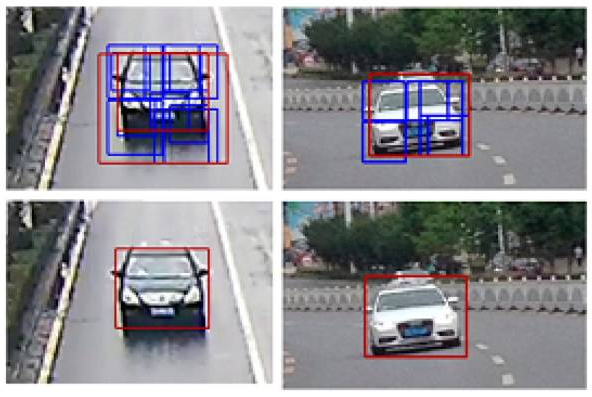
\includegraphics[width=0.5\textwidth]{image007.png}
\caption{Иллюстрация работы метода обнаружения по частям~\cite{ten}}%
\label{fig:how-to-do-research}
\end{figure}

%%%%%%%%%%%%%%%%%%%%%%%%%%%%%%%%%%%%%%%%%%%%%%%%%%%%%%%%%%%%%%%%%%%%%%%%%%%%%%%%
\section{Обнаружение транспортных средств с помощью обучаемых нейросетевых алгоритмов (Learning-Based Detection)}
%%%%%%%%%%%%%%%%%%%%%%%%%%%%%%%%%%%%%%%%%%%%%%%%%%%%%%%%%%%%%%%%%%%%%%%%%%%%%%%%

В основном, подобные алгоритмы основаны на нейронных сетях и требуют предварительного обучения на большом количестве примеров.

В представленной на рисунке ниже схеме даны основные, наиболее распространенные разновидности архитектур искусственных нейронных сетей.

\begin{figure}[htbp]
\centering
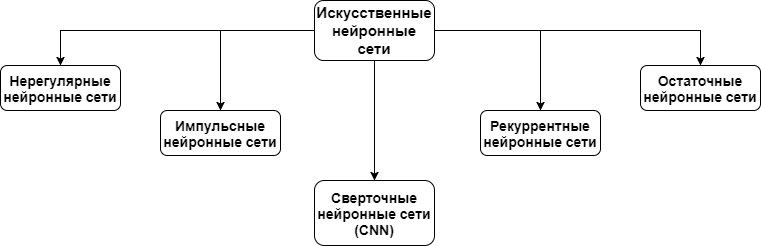
\includegraphics[width=\textwidth]{image008.png}
\caption{Основные архитектуры нейронных сетей}%
\label{fig:how-to-do-research}
\end{figure}

Конкретная разновидность архитектуры нейронной сети выбирается в зависимости от решаемой задачи. Среди наиболее часто используемых типов архитектур выделяют: нерегулярные нейронные сети, импульсные нейронные сети, сверточные нейронные сети, рекуррентные нейронные сети и остаточные нейронные сети. Сверточные нейронные сети являются наиболее часто используемой архитектурой при решении задач технического зрения.

Сверточные нейронные сети, также, как и обычные нейронные сети, состоят из нейронов с обучаемыми весами. Каждый нейрон получает на вход определенное значение, умножает его на весовой коэффициент и преобразует его через нелинейную функцию активации. Однако архитектура подобной сети строится из соображения что на вход подаются пиксели изображения, как показано на рисунке ниже. 

\begin{figure}[htbp]
\centering
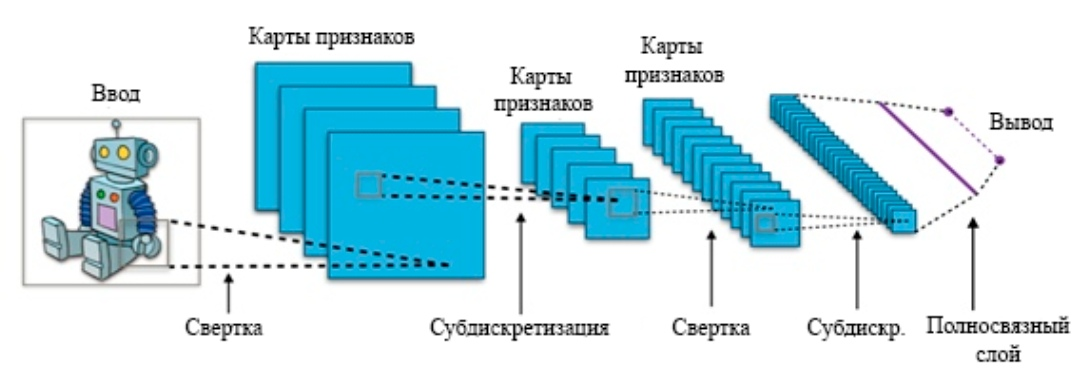
\includegraphics[width=\textwidth]{image009.jpg}
\caption{Архитектура сверточной нейронной сети~\cite{eleven}}%
\label{fig:how-to-do-research}
\end{figure}

Сверточная нейронная сеть характеризуется шириной, высотой и глубиной. Сеть состоит из последовательно расположеных слоёв нейронов, которые выполняют определенные функции. Используются следующие типы слоев и операции: слой свертки, операция субдискретизации и полносвязный слой. Архитектура сверточной нейронной сети строится из последовательно расположенных слоев и операций этих типов.

Сверточные слои реализуют алгебраическую операцию свертки двух матриц. Каждый сверточный слой имеет определенный набор параметров, которые называются фильтрами. Матрица, образованная сверточным слоем, используется для свертки входного изображения и построения карты признаков. Используя несколько фильтров, можно выделить различные признаки во входном изображении. Если последовательно расположить несколько слоев свертки, то можно выделить во входном изображении более высокоуровневые признаки.

Операция субдискретизации (англ. subsampling, англ. pooling, также переводимая как «операция подвыборки» или операция объединения), выполняет уменьшение размерности сформированных карт признаков. В данной архитектуре сети считается, что информация о факте наличия искомого признака важнее точного знания его координат, поэтому из нескольких соседних нейронов карты признаков выбирается максимальный и принимается за один нейрон уплотнённой карты признаков меньшей размерности. За счёт данной операции, помимо ускорения дальнейших вычислений, сеть становится более инвариантной к масштабу входного изображения.

Основная функция полносвязного слоя заключается в использовании построенной карты признаков для определения какому классу эту признаки соответствуют. Количество выходов полносвязного слоя зависит от количества классов, которые умеет обнаруживать данная нейронная сеть~\cite{twelve}.

%%%%%%%%%%%%%%%%%%%%%%%%%%%%%%%%%%%%%%%%%%%%%%%%%%%%%%%%%%%%%%%%%%%%%%%%%%%%%%%%
\subsection{YOLOv3 детектор}
%%%%%%%%%%%%%%%%%%%%%%%%%%%%%%%%%%%%%%%%%%%%%%%%%%%%%%%%%%%%%%%%%%%%%%%%%%%%%%%%

Данная сеть выдвигает гипотезы о четырех координатах для каждой области, где содержится объект. При обучении сети, с помощью этих координат вычисляется ошибка, на основе разницы гипотетических координат и исходных данных. Координаты гипотетической области определяются как те, которые наиболее точно перекрывают область с заданным объектом. Высота и ширина области гипотезы описываются как некоторые отступы от центроида кластера. Координаты центра рассчитываются относительно координат на выходе фильтра после применения к ним сигмоидальной функции.

Во время обучения используется квадратичная функция ошибки для оценки точности сети. В частности, для всех обучающих примеров находится разность между заданными координатами области и полученными на выходе детектора. Сеть также позволяет обрабатывать несколько гипотетических областей, из которых учитывается только та, которая наиболее точно перекрывает исходную область. Если какая-то из гипотез перекрывает заданную область несколько хуже другой гипотезы, то менее точная гипотеза не учитывается, даже если перекрытие области составило выше порогового. 

Каждый участок сетки может содержать области с объектами нескольких классов, что позволяет определять вложенные области, а также объекты пересекающихся классов (например «кошка» и «животное»). В ходе работы детектора гипотезы выдвигаются 3 раза. Таким образом, после получения выходного тензора, содержащего координаты и класс гипотезы, дополнительно используются карты признаков предыдущих слоев (признаки более низкого уровня), которые дополняются картами признаков слоев, идущих за ними. В результате данной операции размер выходного тензора увеличивается. Подобное комбинирование карт признаков с разных стадий свертки позволяет учитывать низкоуровневые признаки полученные на более ранних этапах свертки. 

\begin{figure}[htbp]
\centering
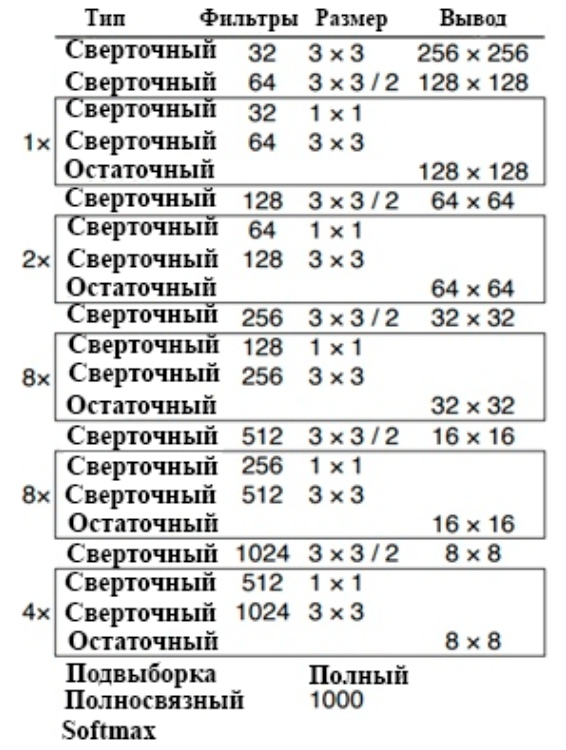
\includegraphics[width=0.5\textwidth]{image010.jpg}
\caption{Экстрактор признаков сети YOLOv3~\cite{thirteen}}%
\label{fig:how-to-do-research}
\end{figure}

Экстрактор признаков данной сети состоит из последовательных сверточных слоев, некоторые из которых соединены напрямую без учета порядка следования. Стоит отметить, что данная сеть имеет более высокое отношение операций с дробными числами к бинарным операциям, что позволяет больше вычислений производить на ~(GPU).
\nomenclature{GPU}{Graphics Processing Unit}
При минимальном пороге пересечения областей равном 0.5 YOLOv3 имеет относительно высокие показатели точности, однако при учете пересечений с коэффициентом больше 0.5 — точность заметно снижается, что позволяет сделать выводы о том, что возникают проблемы с точным выравниванием области гипотезы.

%%%%%%%%%%%%%%%%%%%%%%%%%%%%%%%%%%%%%%%%%%%%%%%%%%%%%%%%%%%%%%%%%%%%%%%%%%%%%%%%
\subsection{SSD детектор}
%%%%%%%%%%%%%%%%%%%%%%%%%%%%%%%%%%%%%%%%%%%%%%%%%%%%%%%%%%%%%%%%%%%%%%%%%%%%%%%%

Основным отличием данной архитектуры детектора является то, что она разрабатывалась специально с учетом необходимости запуска на встраиваемых системах и системах реального времени. В отличие от YOLOv3 в данном подходе не производится повторных ресэмплингов карт признаков для уточнения гипотез. Из-за того, что в данном детекторе отсутствует стадия отбора гипотетических областей — заметен прирост к скорости обнаружения. 

Одной из особенностей является использование небольшого сверточного фильтра для создания гипотез о классе объекта и об отступах области его расположения. Для разных размеров объектов используются отдельные фильтры. Также, эти фильтры применяются к картам признаков более поздних слоев для того, чтобы обеспечить возможность детекции объектов разных размеров и соотношений.

Основные особенности:
%
\begin{itemize*}
  \item Более высокая скорость детекции в сравнении с такими архитектурами как YOLO и Faster R-CNN
  \item Основная идея заключается в создании гипотез содержащих оценку класса объекта и его отступов относительно фиксированного набора изначально заданных областей с помощью небольшого сверточного фильтра
  \item Гипотезы разного масштаба и соотношений размеров производятся с помощью карт признаков разных уровней  
\end{itemize*}
%

На рисунке ниже изображен подход, использующийся для обнаружения объектов в детекторе одного прохода ~(SSD). На рисунке присутствуют два объекта различных размеров и соотношений сторон. Обнаружить первый объект проще на карте признаков \(8x8\), а второй объект на карте признаков \(4x4\). Для каждой гипотетической области оцениваются 4 изначально определенных области с разными соотношениями. Во время обучения сети набор из данных областей сопоставляется областям из обучающего набора. Таким образом, в рамках примера, две гипотетических области для левого объекта и одна для правого объекта будут засчитаны как положительные результаты обнаружения, а остальные — как отрицательные. Функция потерь — это взвешенная сумма потери по локализации объекта и потери по классификации объекта.
\nomenclature{SSD}{Single Shot Detector}

\begin{figure}[htbp]
\centering
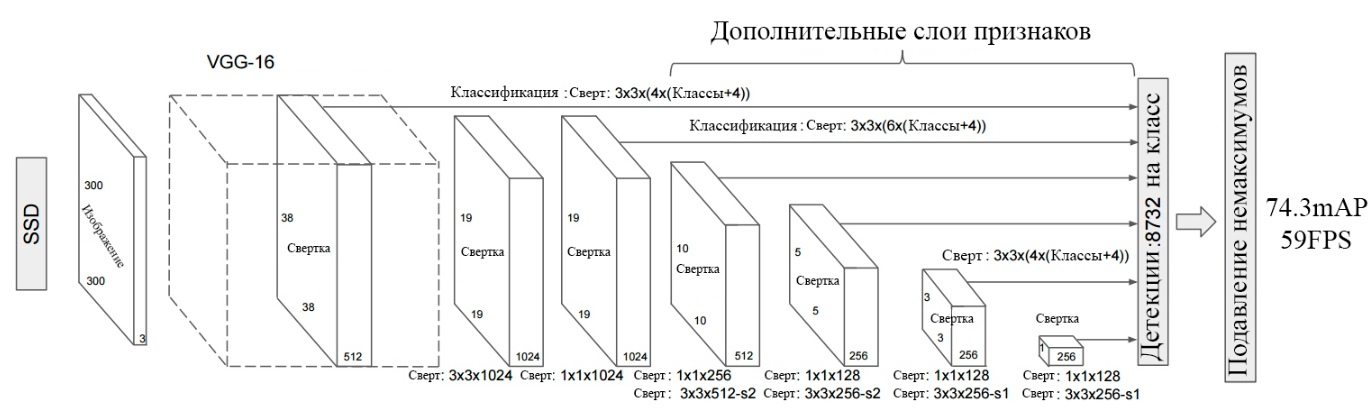
\includegraphics[width=\textwidth]{image011.jpg}
\caption{Архитектура сети SSD\cite{fourteen}}%
\label{fig:how-to-do-research}
\end{figure}

Как видно из рисунка — первые слои состоят из базовой части классификатора VGG-16 с удаленными последними слоями классификации. Дальнейшие сверточные слои служат для построения карт признаков разного масштаба для объектов различных размеров. Каждый из таких слоев производит фиксированное количество гипотез для каждой из областей. Данные сверточные слои образуют последовательные карты признаков разного масштаба, объекты на которых сохраняют свои относительные позиции.

%%%%%%%%%%%%%%%%%%%%%%%%%%%%%%%%%%%%%%%%%%%%%%%%%%%%%%%%%%%%%%%%%%%%%%%%%%%%%%%%
\subsection{Faster R-CNN детектор}
%%%%%%%%%%%%%%%%%%%%%%%%%%%%%%%%%%%%%%%%%%%%%%%%%%%%%%%%%%%%%%%%%%%%%%%%%%%%%%%%

Данная архитектура производит детекцию в несколько этапов. После того как изображение поступило на вход, оно подвергается свертке, а затем подается в сеть извлечения области интересов (Region Proposal Network). Задача данной сети — выдвинуть гипотезы об областях интереса ~(ROI) исходя из данной карты признаков. 
\nomenclature{ROI}{Region Of Interest}
Далее, полученная карта признаков вместе с областями интереса поступает на вход модуля подвыборки, который формирует карты более высокоуровневых признаков и производит классификацию для каждой области интереса. Модуль подвыборки дополнительно делит каждую область интереса на сетку, содержащую множество меньших областей. Таким образом, изначальные области интереса уточняются в ходе подвыборки. 

За основу модели Faster R-CNN была выбрана сеть ImageNet, которая была немного изменена для использования согласно алгоритму, описанному выше. Слои подвыборки максимума были заменены на слои подвыборки областей интереса. Далее, полносвязный слой сети заменен на полносвязные слои для множества категорий объектов и регрессор областей гипотез для каждой из этих категорий.
\begin{figure}[htbp]
\centering
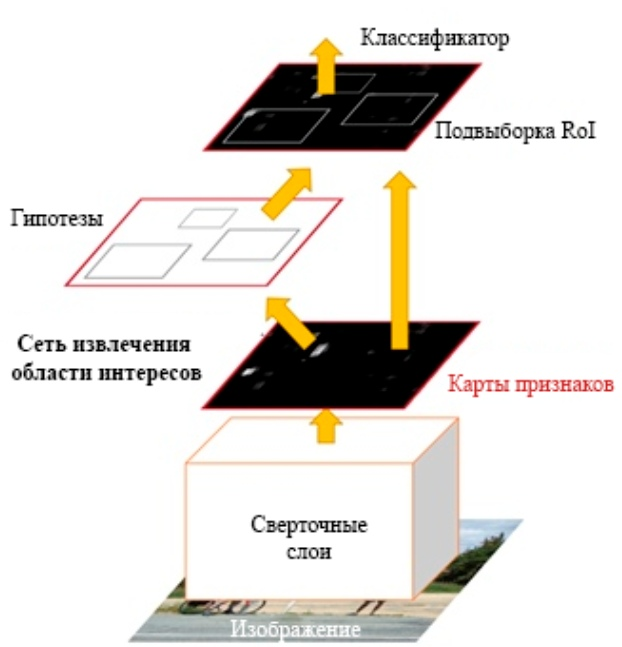
\includegraphics[width=0.5\textwidth]{image012.jpg}
\caption{Архитектура модели Faster R-CNN\cite{fifteen}}%
\label{fig:how-to-do-research}
\end{figure}

%%%%%%%%%%%%%%%%%%%%%%%%%%%%%%%%%%%%%%%%%%%%%%%%%%%%%%%%%%%%%%%%%%%%%%%%%%%%%%%%
\subsection{Mask R-CNN сегментатор}
%%%%%%%%%%%%%%%%%%%%%%%%%%%%%%%%%%%%%%%%%%%%%%%%%%%%%%%%%%%%%%%%%%%%%%%%%%%%%%%%

Данный подход основан на описанной ранее архитектуре Faster R-CNN, с учетом добавления модуля генерации маски сегментации для каждой области интереса (ROI) параллельно с уже существующими модулями классификации и регрессии областей гипотез. 

Модуль для генераии масок представляет из себя полносвязный слой (fully connected layer), который применяется к каждой области интереса, формируя гипотезы содержащие маски сегментации от пикселя к пикселю. Исходная сеть — Faster R-CNN — работает почти идентичным образом, однако она не предназначена для выделения областей с точностью до отдельных пикселей. Для того чтобы это исправить, в Mask R-CNN существует специальный слой квантизации — RoiAlign, который позволяет проводить соответствия между отдельными пикселями в каждой области.

Mask R-CNN (как и Faster R-CNN) можно сформировать из широкого спектра базовых сетей, что позволяет этой системе быть гибкой. Также, архитектура сети производит сегментацию одного кадра за время, равное порядка 200 мс на современном графическом процессоре, что сопоставимо с временем детекции в Faster R-CNN\cite{sixteen}.
\begin{figure}[htbp]
\centering
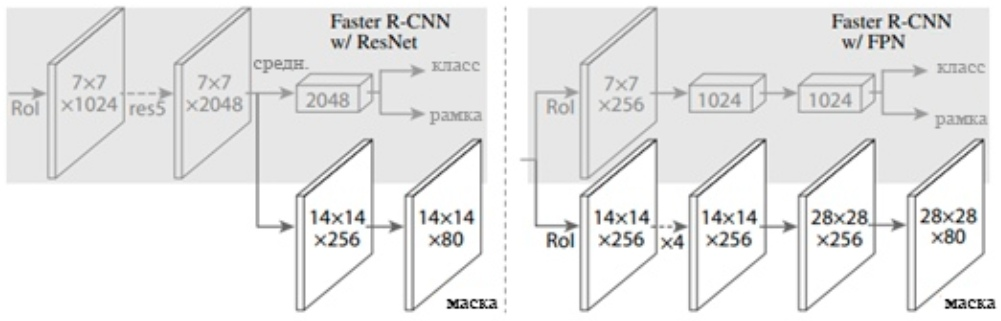
\includegraphics[width=\textwidth]{image013.jpg}
\caption{Архитектура сети Mask R-CNN\cite{sixteen}}%
\label{fig:how-to-do-research}
\end{figure}

%%%%%%%%%%%%%%%%%%%%%%%%%%%%%%%%%%%%%%%%%%%%%%%%%%%%%%%%%%%%%%%%%%%%%%%%%%%%%%%%
\subsection{Сравнительные характеристики представленных моделей}
%%%%%%%%%%%%%%%%%%%%%%%%%%%%%%%%%%%%%%%%%%%%%%%%%%%%%%%%%%%%%%%%%%%%%%%%%%%%%%%%

В данном разделе приведены сравнительные характеристики производительности представленных выше архитектур нейронных сетей. Все измерения проведены на Nvidia Jetson Nano.

Для оценки точности используется показатель средней точности ~(mAP), который определяется как средний показатель точности среди всех представленных классов. Гипотеза считается верной, если пересечение над множеством более или равно 0.5.
\nomenclature{mAP}{Mean Average Precision}

\begin{figure}[htbp]
\centering
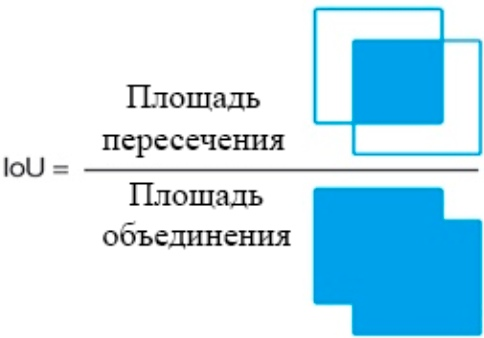
\includegraphics[width=0.35\textwidth]{image014.jpg}
\caption{Расчет пересечения над множеством}%
\label{fig:how-to-do-research}
\end{figure}

Тестовый набор состоит из 850 размеченных вручную изображений в оттенках серого. Изображения созданы путем записи дорожного движения на перекрестке. Исходная выборка была разделена на 3 тестовых подвыборки, иллюстрирующих отдельные ситуации на дорого и положение наблюдаемых объектов относительно камеры:
%
\begin{itemize*}
  \item Плотный поток транспорта от камеры
  \item Плотный поток транспорта в сторону камеры
  \item Ночное двжиение  
\end{itemize*}
%

\begin{figure}[htbp]
\centering
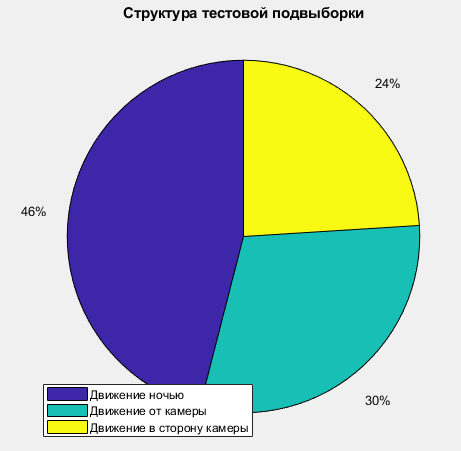
\includegraphics[width=0.5\textwidth]{image015.png}
\caption{Структура тестовой выборки}%
\label{fig:how-to-do-research}
\end{figure}

В таблицах ниже приведены показатели скорости обработки кадра ~(FPS) и точности обнаружения каждой модели, в том числе по каждой тестовой подвыборке отдельно.
\nomenclature{FPS}{Frames Per Second}

\begin{table}[H]
	\caption{Производительность моделей}
	\begin{center}
		\resizebox{\textwidth}{!}{
		\begin{tabular}{|l|c|c|c|l|}
			\hline
			Модель & Конфигурация сети & mAP & FPS & Обучающая выборка \\ \hline
			YOLOv3 & Tiny (320x320) & 0.370 & 32.2 & COCO  \\ \hline
			YOLOv3 & 320x320 & 0.413 & 16.3 & COCO  \\ \hline
			YOLOv3 & 416x416 & 0.520 & 14.2 & COCO  \\ \hline
			YOLOv3 & 608x608 & 0.580 & 11.4 & COCO  \\ \hline
			SSD & 300x300 & 0.451 & 18.2 & 07 + 12 + COCO \\ \hline
			SSD & 512x512 & 0.563 & 15.8 & 07 + 12 + COCO \\ \hline
			Faster R-CNN & 720x720 & 0.528  & 8.5 & VOC 2007 \\ \hline
			Mask R-CNN & 1024x1024 & 0.620 & 4.2 & MS COCO 2017 \\ \hline
		\end{tabular}
		}
		\label{tabular:tab_examp}
	\end{center}
\end{table}

\begin{table}[H]
	\caption{Производительность моделей по каждой подвыборке отдельно}
	\begin{center}
		\resizebox{\textwidth}{!}{
		\begin{tabular}{|l|c|c|c|c|c|}
			\hline
			\multirow{2}{*}{Модель}   & \multirow{2}{*}{Конфигурация}   & \multicolumn{4}{c|}{Точность на подвыборке, mAP} \\ \cline{3-6} 
									  &     & Смешанная   & В сторону камеры    & Ночная	 & От камеры   \\ \hline
						YOLOv3			  & Tiny (320x320)    & 0.370    & 0.483    & 0.273   & 0.333	\\ \hline
						YOLOv3			  & 320x320    & 0.413    & 0.553    & 0.366   & 0.433	\\ \hline
						YOLOv3			  &  416x416   & 0.520    & 0.573    & 0.460   & 0.543	\\ \hline
						YOLOv3			  &  608x608   & 0.580    & 0.620    & 0.486   & 0.586	\\ \hline
						SSD			  & 300x300    & 0.451    & 0.577    & 0.302   & 0.447	\\ \hline
						SSD			  & 512x512    & 0.563    & 0.688    & 0.358   & 0.483	\\ \hline
						Faster R-CNN	& 720x720    & 0.528    & 0.562    & 0.425   & 0.465	\\ \hline
						Faster R-CNN	& 1024x1024    & 0.620    & 0.696    & 0.335   & 0.547	\\ \hline
									  
		\end{tabular}
		}
		\label{tabular:tab_examp}
	\end{center}
\end{table}

\begin{figure}[htbp]
\centering
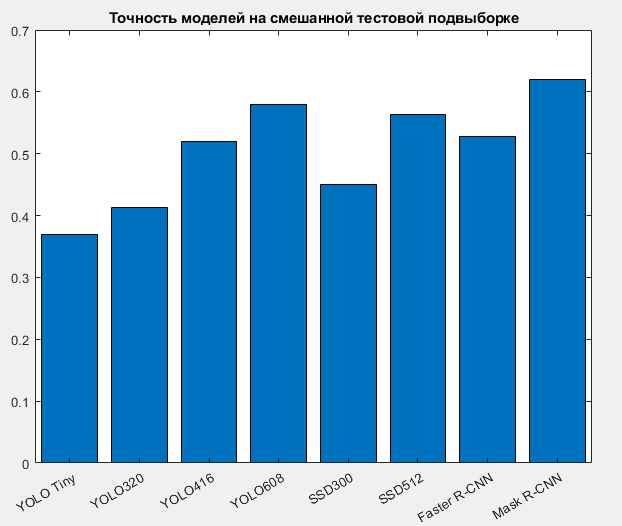
\includegraphics[width=0.5\textwidth]{image016.png}
\caption{График точности представленных моделей на смешанной тестовой подвыборке}%
\label{fig:how-to-do-research}
\end{figure}

\begin{figure}[htbp]
\centering
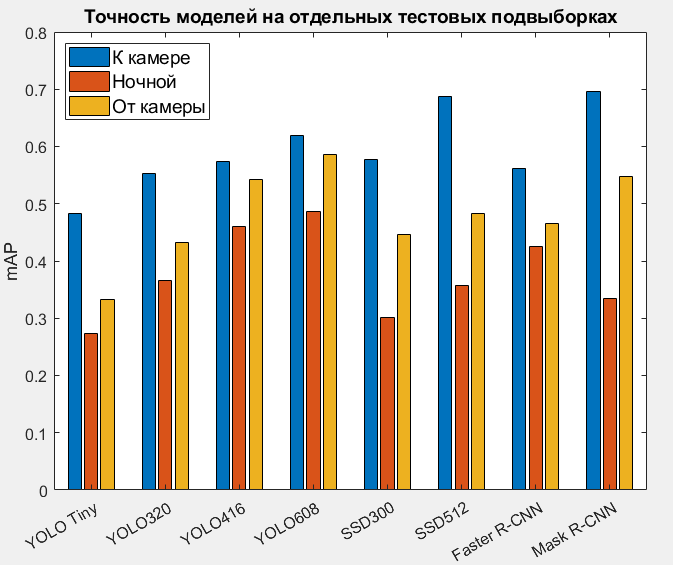
\includegraphics[width=0.5\textwidth]{image017.png}
\caption{Точность моделей на отдельных тестовых подвыборках}%
\label{fig:how-to-do-research}
\end{figure}

%%%%%%%%%%%%%%%%%%%%%%%%%%%%%%%%%%%%%%%%%%%%%%%%%%%%%%%%%%%%%%%%%%%%%%%%%%%%%%%%
\section{Анализ используемых при разработке средств, инструментов и методов}
%%%%%%%%%%%%%%%%%%%%%%%%%%%%%%%%%%%%%%%%%%%%%%%%%%%%%%%%%%%%%%%%%%%%%%%%%%%%%%%%

%%%%%%%%%%%%%%%%%%%%%%%%%%%%%%%%%%%%%%%%%%%%%%%%%%%%%%%%%%%%%%%%%%%%%%%%%%%%%%%%
\subsection{Анализ и выбор среды и языка разработки}
%%%%%%%%%%%%%%%%%%%%%%%%%%%%%%%%%%%%%%%%%%%%%%%%%%%%%%%%%%%%%%%%%%%%%%%%%%%%%%%%

В качестве среды разработки рассматривается PyCharm от JetBrains. Данная среда разработки ориентирована на создание систем на Python и позволяет удобно и быстро настраивать большие Python-проекты. 

В качестве версии Python была выбрана версия 3.7.3, которая необходима для работы TensorFlow.

%%%%%%%%%%%%%%%%%%%%%%%%%%%%%%%%%%%%%%%%%%%%%%%%%%%%%%%%%%%%%%%%%%%%%%%%%%%%%%%%
\subsection{Анализ инструментов системы обучения}
%%%%%%%%%%%%%%%%%%%%%%%%%%%%%%%%%%%%%%%%%%%%%%%%%%%%%%%%%%%%%%%%%%%%%%%%%%%%%%%%

%%%%%%%%%%%%%%%%%%%%%%%%%%%%%%%%%%%%%%%%%%%%%%%%%%%%%%%%%%%%%%%%%%%%%%%%%%%%%%%%
\subsubsection{Библиотека глубокого обучения TensorFlow}
%%%%%%%%%%%%%%%%%%%%%%%%%%%%%%%%%%%%%%%%%%%%%%%%%%%%%%%%%%%%%%%%%%%%%%%%%%%%%%%%

TensorFlow — открытая программная библиотека для машинного обучения, разработанная компанией Google для решения задач построения и обучения нейронной сети с целью автоматического нахождения и классификации образов. Применяется как для исследований, так и для разработки собственных продуктов Google. Основной API для работы с библиотекой реализован для Python. Нацелена на оперативную работу с сетями глубинного обучения, при этом спроектирована так, чтобы быть компактной, модульной и расширяемой. TensorFlow предоставляет высокоуровневый набор абстракций, который делает простым формирование нейронных сетей, их обучение и использование.

TensorFlow имеет ряд зависимостей от сторонних пакетов для работы:
%
\begin{itemize*}
  \item numpy – пакет, поддерживающий работу с многомерными массивами и матрицами, а также с математическими функциями. Библиотека NumPy предоставляет реализации вычислительных алгоритмов (в виде функций и операторов), оптимизированные для работы с многомерными массивами. В результате любой алгоритм, который может быть выражен в виде последовательности операций над массивами (матрицами) и реализованный с использованием NumPy, работает так же быстро, как эквивалентный код, выполняемый в MATLAB
  \item scipy – библиотека для языка программирования Python с открытым исходным кодом, предназначенная для выполнения научных и инженерных расчётов. Имеет возможности для поиска минимумов и максимумов функций, вычисления интегралов функций, поддержки специальных функций, обработки сигналов, обработки изображений
  \item scikit-learn – набор алгоритмов машинного обучения с учителем и без учителя. Широко используется для промышленных систем, в которых применяются алгоритмы классического машинного обучения. Scikit-learn специализируется на алгоритмах машинного обучения для решения задач обучения с учителем: классификации (предсказание признака, множество допустимых значений которого ограничено) и регрессии (предсказание признака с вещественными значениями), а также для задач обучения без учителя: кластеризации (разбиение данных по классам, которые модель определит сама), понижения размерности (представление данных в пространстве меньшей размерности с минимальными потерями полезной информации) и детектирования аномалий  
\end{itemize*}
%

Модель в TensorFlow представляет собой последовательность или граф автономных модулей, которые соединяются между собой, как детали, образуя нейронную сеть. В библиотеке имеется множество готовых моделей, реализующих различные типы слоев, функций стоимости, оптимизаторов, схем инициализации, функций активации и методов регуляризации.

%%%%%%%%%%%%%%%%%%%%%%%%%%%%%%%%%%%%%%%%%%%%%%%%%%%%%%%%%%%%%%%%%%%%%%%%%%%%%%%%
\subsubsection{Инструменты анализа обучения сети TensorBoard}
%%%%%%%%%%%%%%%%%%%%%%%%%%%%%%%%%%%%%%%%%%%%%%%%%%%%%%%%%%%%%%%%%%%%%%%%%%%%%%%%

При использовании библиотеки Tensorflow есть возможность использования инструментов анализа обучения сети. Данный набор инструментов позволяет в простой форме представить качественные характеристики обучения нейронной сети как функцию от времени. 

Для использования данного инструментария в реализованной программе, необходимо добавить в проект функцию, позволяющую в потоковом режиме записывать текущие параметры сети в отдельный файл. По мере того, как сеть обучается, файл с параметрами постоянно перезаписывается. Для того, чтобы визуализировать содержимое файла достаточно передать его на обработку в установленный пакет TensorBoard. После того как обработка содержимого файла завершается, визуализированные графики можно увидеть через браузер по локальному адресу localhost:6006.

Этот пакет инструментов позволяет визуализировать такие характеристики нейронной сети как:
%
\begin{itemize*}
  \item Точность обнаружения сети на обучающем наборе
  \item Величина функции ошибки при обработке обучающего набора
  \item Точность обнаружения сети на наборе валидации
  \item Величина функции ошибки при обработке набора валидации
\end{itemize*}
%

\begin{figure}[htbp]
\centering
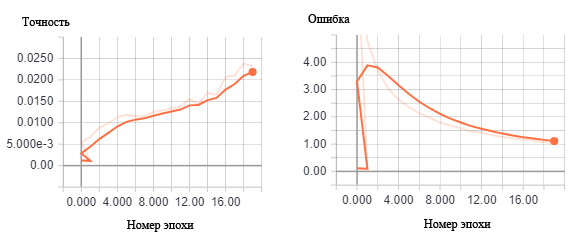
\includegraphics[width=0.5\textwidth]{image018.jpg}
\caption{Пример визуализации обучения с помощью TensorBoard}%
\label{fig:how-to-do-research}
\end{figure}

%%%%%%%%%%%%%%%%%%%%%%%%%%%%%%%%%%%%%%%%%%%%%%%%%%%%%%%%%%%%%%%%%%%%%%%%%%%%%%%%
\subsubsection{Средства и методы формирования обучающего набора}
%%%%%%%%%%%%%%%%%%%%%%%%%%%%%%%%%%%%%%%%%%%%%%%%%%%%%%%%%%%%%%%%%%%%%%%%%%%%%%%%

Вся информация, которую нейронная сеть будет иметь о задаче, содержится в наборе обучающих примеров. Поэтому качество обучения нейронной сети напрямую зависит от количества и качества примеров в обучающей выборке, а также от того, насколько полно эти примеры описывают данную предметную область. 

При создании систем детектирования изображения на основе нейронных сетей в первую очередь необходимо создание обучающей выборки, максимально охватывающей все множество естественных данных.

В качестве учебного набора в данной работе используется большой набор изображений, полученных из различных источников. В процессе сбора изображений транспортных средств выполнялась задача обеспечения нейронной сети эффективным набором изображений, полученных в различных условиях съемки.

Скользящий контроль или кросс-проверка или кросс-валидация (cross-validation) — процедура эмпирического оценивания обобщающей способности алгоритмов, обучаемых по прецедентам.

Фиксируется некоторое множество разбиений исходной выборки на две подвыборки: обучающую и контрольную. Для каждого разбиения выполняется настройка алгоритма по обучающей подвыборке, затем оценивается его средняя ошибка на объектах контрольной подвыборки. Оценкой скользящего контроля называется средняя по всем разбиениям величина ошибки на контрольных подвыборках.

Если выборка независима, то средняя ошибка скользящего контроля даёт несмещённую оценку вероятности ошибки. Это выгодно отличает её от средней ошибки на обучающей выборке, которая может оказаться смещённой (оптимистически заниженной) оценкой вероятности ошибки, что связано с явлением переобучения.

Скользящий контроль является стандартной методикой тестирования и сравнения алгоритмов классификации, регрессии и прогнозирования.

%%%%%%%%%%%%%%%%%%%%%%%%%%%%%%%%%%%%%%%%%%%%%%%%%%%%%%%%%%%%%%%%%%%%%%%%%%%%%%%%
\subsection{Анализ инструментов встраиваемой системы}
%%%%%%%%%%%%%%%%%%%%%%%%%%%%%%%%%%%%%%%%%%%%%%%%%%%%%%%%%%%%%%%%%%%%%%%%%%%%%%%%

%%%%%%%%%%%%%%%%%%%%%%%%%%%%%%%%%%%%%%%%%%%%%%%%%%%%%%%%%%%%%%%%%%%%%%%%%%%%%%%%
\subsubsection{Физические характеристики}
%%%%%%%%%%%%%%%%%%%%%%%%%%%%%%%%%%%%%%%%%%%%%%%%%%%%%%%%%%%%%%%%%%%%%%%%%%%%%%%%

Nvidia Jetson Nano – это встраиваемый вычислительный модуль, обеспечивающий значительную производительность при развертывании компонент систем машинного обучения.  Представляет собой модуль размером 70 x 45 мм и является самым компактным устройством в линейке Jetson.

Спецификации встраиваемого устройства:

\begin{table}[H]
	\caption{Спецификации Jetson Nano}
	\begin{center}
		\resizebox{\textwidth}{!}{
		\begin{tabular}{|l|l|}
			\hline
			Видеокарта & Maxwell со 128 ядрами \\ \hline
			Процессор & Четырехъядерный ARM A57 с частотой 1.43 ГГц \\ \hline
			Память & 4 Гб LPDDR4, 64-bit 25.6 Гбит/с \\ \hline
			Флэш-память & microSD \\ \hline
			\multirow{3}{*}{Кодирование видео} & 4К с частотой 30 Гц, 4 потока в разрешении 1080p  \\ 
											&	 с частотой 30 Гц, 9 потоков в разрешении 720p с частотой 30 Гц,	\\
												&  в форматах H. 264/H. 265				\\ \hline
			\multirow{3}{*}{Декодирование видео} & 4К с частотой 60 Гц, 2 потока в разрешении 4K  \\ 
												&	с частотой 30 Гц, 8 потоков в разрешении 1080p с частотой 30 Гц, \\ 
												& 18 потоков в разрешении 720p с частотой 30 Гц, в форматах H.264/H.265\\ \hline
			Камера & 2 полосы MIPI CSI-2 DPHY \\ \hline
			Подключение & Gigabit Ethernet, M.2 Key E \\ \hline
			Дисплей & HDMI и DP \\ \hline
			USB & 4x USB 3.0, USB 2.0 Micro-B \\ \hline
			Прочие характеристики & GPIO, I2C, I2S, SPI, UART \\ \hline
		\end{tabular}
		}
		\label{tabular:tab_examp}
	\end{center}
\end{table}

%%%%%%%%%%%%%%%%%%%%%%%%%%%%%%%%%%%%%%%%%%%%%%%%%%%%%%%%%%%%%%%%%%%%%%%%%%%%%%%%
\subsubsection{Набор программных инструментов}
%%%%%%%%%%%%%%%%%%%%%%%%%%%%%%%%%%%%%%%%%%%%%%%%%%%%%%%%%%%%%%%%%%%%%%%%%%%%%%%%

Операционная система Nvidia Jetson Nano – Linux For Tegra ~(L4T), которая включена в пакет для разработки под названием JetPack. Вместе с операционной системой, пакет для разработки включает в себя следующие ключевые компоненты:
\nomenclature{L4T}{Linux For Tegra}

%
\begin{itemize*}
  \item TensorRT.
	Программный ускоритель для выполнения вычислений задач машинного обучения. Включает в себя оптимизатор моделей глубокого обучения, а также среду выполнения, которая предоставляет низкую задержку и высокую производительность для программ машинного обучения.
	В качестве оптимизации данный модуль позволяет выполнить уменьшение разрядности параметров сети (INT 8 или FP16) и регуляризацию слоев. Это позволяет снизить вычислительную сложность модели во время выполнения. 
	В контексте данной работы TensorRT использовался для оптимизации и запуска модели, обученной с помощью TensorFlow.
	\begin{figure}[htbp]
	\centering
	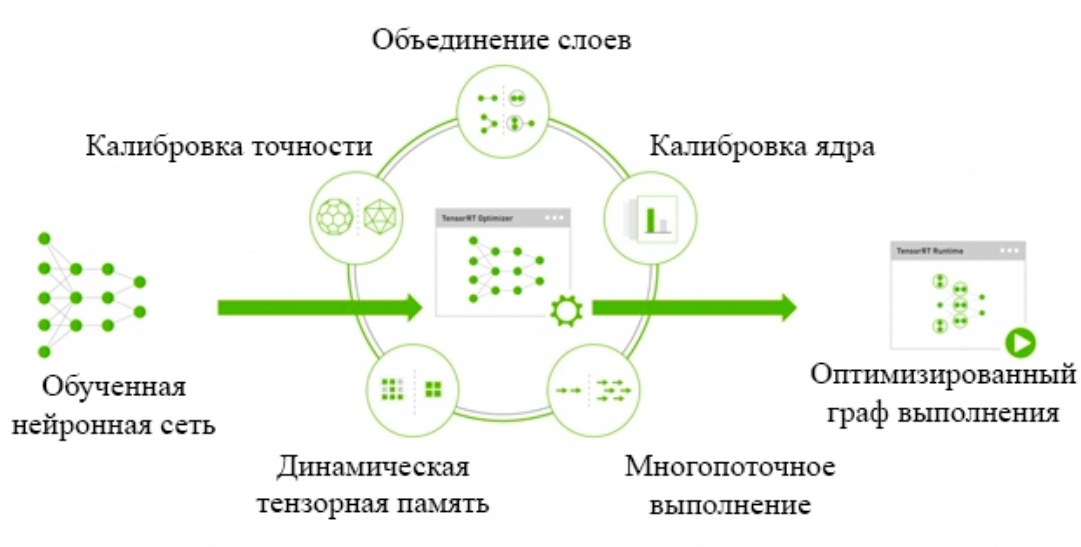
\includegraphics[width=\textwidth]{image019.jpg}
	\caption{Компоненты TensorRT}%
	\label{fig:how-to-do-research}
	\end{figure}
  \item cuDNN.
	Библиотека примитивов для вычислений, связанных с машинным обучением. Предоставляет методы для свертки, подвыборки, нормализации и активации, оптимизированные под графический процессор.
  \item OpenCV.
	Библиотека примитивов, содержащая методы обработки изображений и покадровой работы с потоками видео.	
  \item DeepStream.
	Фреймворк, содержащий плагины, позволяющие интегрировать модули глубокого обучения в потоковую систему, обеспечивая низкую задержку на кодирование и декодирование видео.
\end{itemize*}
%

%%%%%%%%%%%%%%%%%%%%%%%%%%%%%%%%%%%%%%%%%%%%%%%%%%%%%%%%%%%%%%%%%%%%%%%%%%%%%%%%
\section{Выводы по разделу}
%%%%%%%%%%%%%%%%%%%%%%%%%%%%%%%%%%%%%%%%%%%%%%%%%%%%%%%%%%%%%%%%%%%%%%%%%%%%%%%%

По соотношению скорости обработки и устойчивости – обучаемые нейросетевые алгоритмы являются наиболее оптимальным вариантом для реализации детектора. Обнаружение объектов по моделям обладает существенными недостатками по сравнению с другими методами. Он требует составления большой базы моделей транспортных средств, и описания этих моделей с помощью геометрических примитивов. С учетом того, что некоторые типы транспортных средств могут быть очень похожи друг на друга – геометрические примитивы могут быть очень сложные для решения поставленной в этой работе задачи. Для реализации детектора на основе методов, представленных в разделе 1.2, необходимо изначально определить способ представления признаков объекта, а затем выполнить классификацию, с помощью метода опорных векторов. Обучаемые нейросетевые алгоритмы позволяют не определять признаки строго, так как основаны на сверточных нейронных сетях. Исходя из этого, в контексте данной работы было решено использовать нейросетевой подход для реализации системы обнаружения.

По итогам обработки представленных выше результатов можно сделать вывод о том, что точность обнаружения рассматриваемых решений зависит не только от выбранной архитектуры и размерности входного изображения, но также и от сложившейся на дороге ситуации. Наибольшую точность и устойчивость к изменяющимся ситуациям показали решения на основе архитектуры SSD. Несмотря на то, что точность обнаружения решения на основе Faster R-CNN показало более низкую точность, оно тоже оказалось устойчивым к различным дорожным ситуациям. 

Принимая во внимание скорость обработки кадра (FPS), можно также сделать вывод о том, что решение SSD обладает оптимальным соотношением скорости и точности обнаружения. Так как архитектура данной сети построена с учетом распознавания цветных изображений – существует возможность дополнительного увеличения производительности при снижении количества каналов входного изображения до одного.

Несмотря на это, SSD показывает не столь хорошие результаты обнаружения при попытке распознать автомобиль сзади, что требует дополнительной доработки. Также, ни одно из рассмотренных выше решений не удовлетворяет требованиям по количеству необходимых для распознавания классов, представленных в функциональных требованиях. 

\iffalse
\begin{table}[H]
	\caption{Название таблицы}
	\begin{center}
		\begin{tabular}{|l|l|}
			\hline
			top left & top right\\ \hline
			bot left & bot right\\ \hline
		\end{tabular}
		\label{tabular:tab_examp}
	\end{center}
\end{table}
\fi

